\section{Methods}
The goal is to identify the measurement settings from which one can extract kinetic information captured in a CV response.
Towards this goal, we seek to identify measurement conditions for which an S-shape CV curve is collected by our oracle. 
An active learning technique summarized in~\Cref{fig:workflow} is used to accelerate the search for measurement settings within fixed computational budget. 
The active learning approach involves iterative collection of data points from a search space \(\mathcal{S}\).
The process starts with a small set of observed data \(D=(\textbf{S},\textbf{Y})\) where \(\textbf{S}\in\mathcal{S}\) are the observed locations and \(\textbf{Y}\in\{-1,1\}\) are corresponding labels. 
In each iteration, the algorithm collects data and incrementally updates the decision model \(p(y=+1|D)\) it aims to learn with \(y\) representing a label.
A user-defined selector~(or policy) identifies a~(or a batch of) candidate location(s) in the search space for observing the next response.
The policy typically maximizes a utility function given the decision model. 
For example, given \(D\), we can define a policy using a utility function that simply counts number of targets in the dataset \(u(\textbf{S})=\sum\limits_{s_i\in \textbf{S}, y_i \in \textbf{Y}} [y_i=+1]\). 
A policy can be defined to select more targets to be added to the data pool \(D\) using: 
\begin{equation}
    s^* = \argmax_s \mathbb{E}\left[ u(\mathcal{S} \setminus \textbf{S} | D )\right] 
    \label{eq:policy}
\end{equation}
Given a location \(s^* \in\mathcal{S}\), the corresponding experiment is performed and a response is collected. 
In this chapter, a CV response curve is collected from a CV curve simulator and the response is then passed onto an oracle. 
Oracle labels the response to be either a target or non-target~(for example in~\Cref{fig:workflow}, we show a non-target like CV shape which will be  assigned \(y^*=-1\) as a label). 
The next step is to augment \(D\) using the data collected in the current iteration i.e. \(D^* = D\cup (s^*,y^*) \). 
The decision model is then updated with \(D^*\). 
This process is repeated until the computational budget--defined in terms of total number of label queries or equivalently number of simulations--is exhausted.
As an oracle we use a Bayesian Model Selection (BMS) that operates on two models \(\mathcal{M}_1, \mathcal{M}_2\) referred to as null model~(representing a typical CV curve) and target model~(representing an S-shaped CV curve), respectively.
Moreover, we use a variation of active learning called active search~\cite{garnett2012bayesian} which maximizes the number of targets found in contrast to traditional active learning where the selector is defined with a goal to closely approximate \(p(y=+1\vert D )\).


\begin{figure}[h]
    \centering
    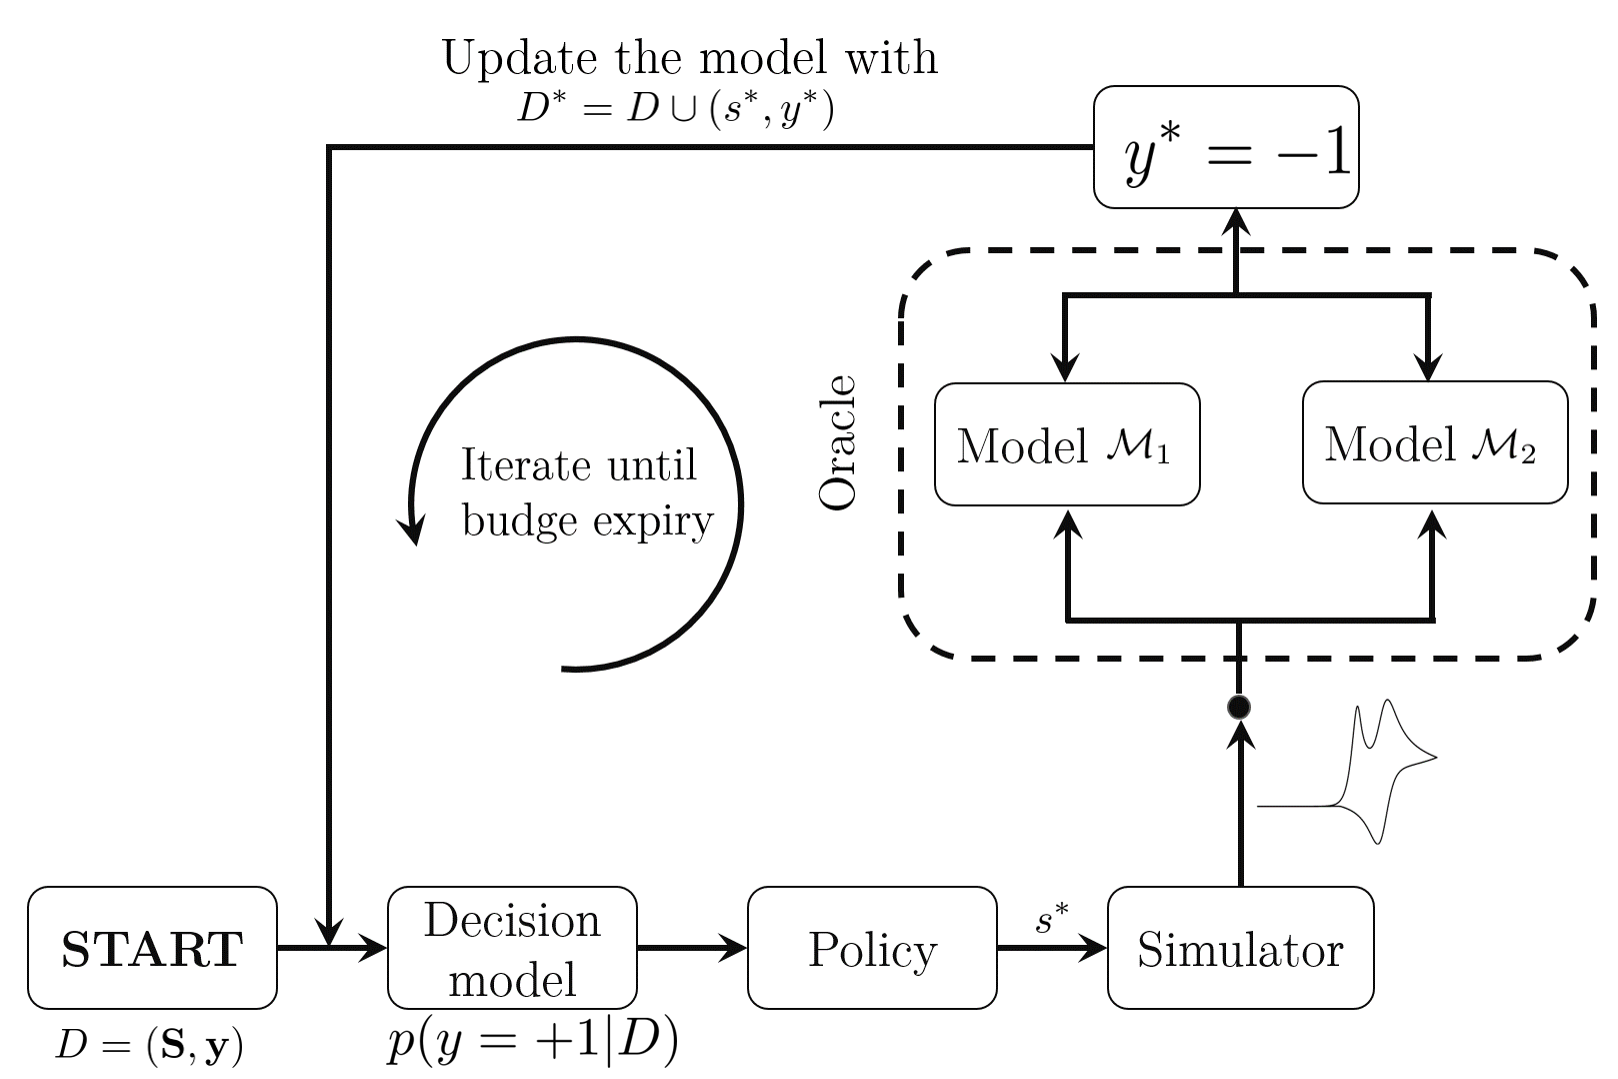
\includegraphics[width=0.75\linewidth]{Chapter-3/figures/workflow_gpcv.png}
    \caption{Active learning framework as a flowchart. Active learning iterations start with a few labelled data points in the search space \(\mathcal{S}\). We stop collecting data when we have selected a pre-defined number (called budget) of locations for updating our decision (or belief) model.}
    \label{fig:workflow}
\end{figure}
